\documentclass[11pt,a4paper]{article} % ,titlepage
\usepackage{fontspec}
\usepackage{parskip}
\usepackage{algorithm}
\usepackage{algorithmic}
% This is now the recommended way for checking for PDFLaTeX:
\usepackage{ifpdf}
\ifpdf
\usepackage[pdftex]{graphicx}
\else
\usepackage{graphicx}
\fi

\algsetup{indent=2em} 
\newcommand{\factorial}{\ensuremath{\mbox{\sc Factorial}}}

\defaultfontfeatures{Scale=MatchLowercase}

% \usepackage{bookman}

% \setmainfont[Mapping=tex-text]{Gentium Basic}%Gentium Basic} % Heofler Text
% \setsansfont[Mapping=tex-text]{Optima}
% \setmonofont{Bitstream Vera Sans Mono}\title{}

\setlength{\parindent}{20pt}
\setlength{\parskip}{2ex}

\title{Recommender agents}
\author{Prodan Andrei-Cristian \\ 
		Master, II$^{nd}$ year, group 256 \\
		\texttt{prodan.cristian@gmail.com}}

\begin{document}

\maketitle

% \newpage

\begin{abstract}
This documents presents a multiagent system which represents a recommender system for a user. The idea is that the user connects to (has) an AssistentAgent. This agent will then collaborate with other types of agents (RecommenderAgent, InformationAgent) and an environment in order to provide the users with different recommendations, in a distributed manner. The software is implemented in the Ruby programming language, using only it's standard API. For this software we make expensive use of the DRb (Distributed Ruby) module.
\end{abstract}


\section{Project description}
This software implements the multiagent paradigm in a distributed manner. The software (which we will refer to by the name of ReCo) serves as a distributed environment for recommending movies to a user. There are mainly two functions of this system from the user perspective that is:
\begin{itemize}
    \item get some recommendations for me (the user);
    \item set rating $x$ for movie $y$ on behalf of me (the user);
\end{itemize}

Inside the software this functions have the following signature. 
\begin{verbatim}
    get_recommendations(user_id)
    
    set_recommendation(user_id, movie_id, rating)
\end{verbatim}

The actual method for the recommendation is collaborative filtering. This technique makes use of triples like $<movie_{id}, rating_{id}, user_{id}>$ in order to compute recommendations for users. It relies of the fact that if two users have agreed upon certain preferences in the past, it is very likely to have the same preferences in the future. There are several methods that can be used to compute similarities between the users: neighborhood methods (Pearson coefficient) or latent factors decomposition. 

Because this software focuses the design of agents none of the actual algorithms for the recommendation have been implemented. We only state some of the potential methods for doing this. Right now, we have placed some stubs methods which wait for a random number of milliseconds and return a random result. The usefulness of this software could be justified by this.

Figure \ref{fig:arch} shows the architecture of the system. We analyze each component in the next step.

\begin{figure}
    \begin{center}
        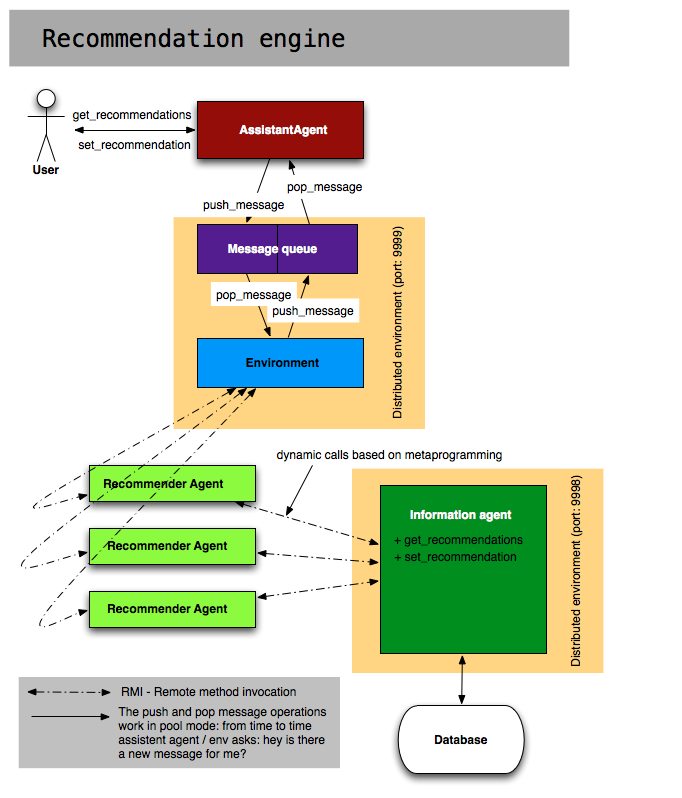
\includegraphics[scale=0.7]{architecture}
        \caption{\small{ReCo architecture}\label{fig:arch}}
    \end{center}
\end{figure}

\begin{itemize}
    \item \textbf{AssistantAgent} (AssistantAgent.rb). This agent communicates with the users. It exposes two interfaces for getting and setting recommendations (details on figure \ref{fig:classes}). 
    
    \item \textbf{The environment} (environment.rb). Is a service which shares a \textsc{MessageQueue} object with different agents. It is the layer that makes the communication possible between the \textsc{AssistantAgent} and the \textsc{InformationAgent}. Each time he has to respond to a query (which he takes from the queue, in form of a message), he ``sends'' a \textsc{RecommenderAgent} to \textsc{ask} the \textsc{InformationAgent} some info based on the query. The \textsc{RecommenderAgent} does this using Remote Method Invocation. By chaining all these calling methods, the environment gets back the answer and puts it into the queue again but in a form of an answer (they will be then used by the \textsc{AssistantAgent} as an answer to their initial query).
    
    \item \textbf{The InformationAgent} (InformationAgent.rb). This agent runs like a standalone service. He waits for it's methods to be called using RMI by the \textsc{RecommenderAgent}. It's methods can be seen in figure \ref{fig:classes}.
    
    \item \textbf{The RecommenderAgent} (RecommenderAgent.rb). This agent is instantiated by the environment and ``sent'' to ask the \textsc{InformationAgent} to solve it's query. It has only one ask method but other things might be implemented here.
    
    \item \textbf{The message queue}. The message queue holds messages which can be of type ``question'' and ``answer'' and represent communication messages between the \textsc{AssistantAgent} and the \textsc{environment}. More on this can be read about in the next chapter. The mechanism for communication between agents is \textbf{asynchronous message passing}.
\end{itemize}


\section{Implementation}
This piece of software has been implemented using DRb module which can be found in the standard API of the Ruby distribution. 

DRb allows Ruby programs to communicate with each other on the same machine or over a network. DRb uses remote method invocation (RMI) to pass commands and data between processes.

The \textsc{environment} starts as a service at port 9999 and exposes a queue. This queue is shared with different \textsc{AssistentAgents} that need to use the recommendation engine. From time to time, the environment looks through the queue (pool) to see if there are any new messages. If there are, it takes them and sends them to the \textsc{RecommenderAgent}. This Agent is instantiated in the \textsc{environment} and calls the \textsc{askInformation} method on the InformationAgent. The param to it's query is a \textsc{message}. Based on that \textsc{message}, the InformationAgent, which runs at port 9998 can figure which kind of info the \textsc{RecommenderAgent} needs (weather it is \textsc{get\_recommendation} or \textsc{set\_recommendation} ).

In this time the \textsc{AssistantAgent} waits for it\'s response. It does this by checking from time to time the shared queue. He basically asks: ``hey is there any new message for me''.

A message contains the info shown in figure \ref{fig:classes}. The \textsc{kind} field can be ``Q'' or ``A'' weather the message refers from a query of an agent or a response of the environment respectively. The \textsc{type} field may be: \textsc{GET\_RECOMMENDATIONS} or \textsc{SET\_RECOMMENDATION} and this is used by the \textsc{InformationAgent} to figure out what type of query should he respond. The params field contains a Hash with params like: \textsc{user\_id}, \textsc{movie\_id}, \textsc{rating} or \textsc{agent\_id}.

The classes which form the system are shown in figure \ref{fig:classes}.

\begin{figure}
    \begin{center}
        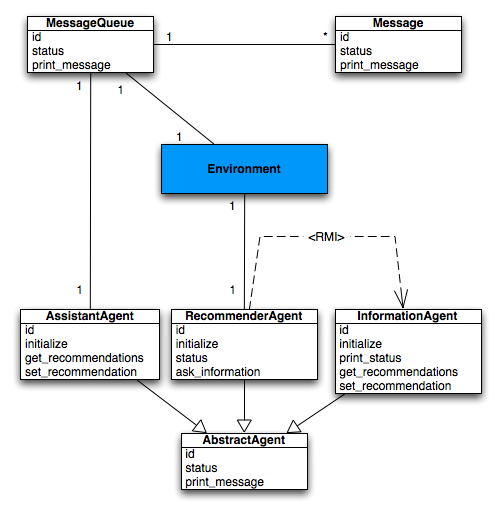
\includegraphics[scale=0.5]{classes}
        \caption{\small{ReCo classes}\label{fig:classes}}
    \end{center}
\end{figure}

\section{Demonstration}

In order to be able to test the system Ruby 1.8 has to be installed on the system. The standard installation for Ruby contains the DRb system.

The simluation.rb file contains a simulation for this system. The file is quite intuitive and can easily be modified. It spawns 10 threads and each thread initializes one agents which make two recommendation requests.

From the command line, go to the root directory of the software. First make sure all the necessary files have execution rights (not necessary on windows). This can be done using the following commands (Linux, MacOS):

\begin{verbatim}
    chmod +x simulation.rb
    chmod +x InformationAgent.rb
    chmod +x environment.rb
\end{verbatim}

Then run:
\begin{verbatim}
    ./InformationAgent.rb
    ./environment.rb
    ./simulation.rb
\end{verbatim}

On a MacOs Machine this should show something like the screens in figure \ref{fig:screens}.

\begin{figure}
    \begin{center}
        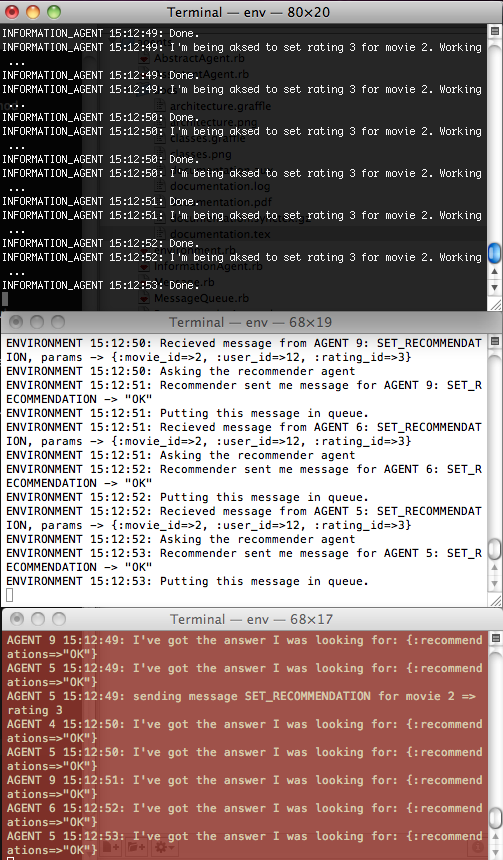
\includegraphics[scale=0.6]{screens}
        \caption{\small{ReCo demo}\label{fig:screens}}
    \end{center}
\end{figure}


% \bibliographystyle{plain}
% \bibliography{referat}

\end{document}
